% fig_hpr_bound: the high point relaxation (HPR) sandwich used for the
% MIPLIB-derived instances.  The HPR drops the follower's optimality, so its
% optimum (= the published MIPLIB optimum, checked exactly by
% scripts/compare_hpr.py) is a lower bound on the bilevel optimum; any verified
% bilevel feasible point is an upper bound.  When the two meet, the point is
% optimal.  Schematic (no data).
% Build: pdflatex fig_hpr_bound.tex   (3.15 in x 1 in)
\documentclass[tikz,border=2pt]{standalone}
\pdfinfoomitdate=1 \pdftrailerid{} \pdfsuppressptexinfo=-1 % byte-identical rebuilds
\usepackage{mathptmx}
\usetikzlibrary{arrows.meta,calc,decorations.pathreplacing,shapes.geometric}
\definecolor{leader}{HTML}{2A78D6}
\definecolor{follower}{HTML}{EB6834}
\definecolor{cert}{HTML}{1BAF7A}
\definecolor{ink}{HTML}{0B0B0B}
\definecolor{ink2}{HTML}{52514E}
\definecolor{muted}{HTML}{A9A8A2}
\definecolor{grid}{HTML}{E6E5E0}
\tikzset{
  every picture/.style={font=\fontsize{8}{9.6}\selectfont, color=ink, line cap=round},
  small/.style={font=\fontsize{7}{8.4}\selectfont},
  lab/.style={anchor=south, align=center, inner sep=1pt},
}
\begin{document}
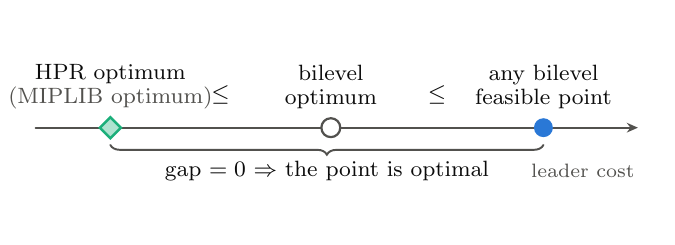
\begin{tikzpicture}
  % fixed page: 3.15 in x 1 in including the 2 pt border
  \useasboundingbox (0,0) rectangle (7.86,2.40);
  \def\y{1.13}
  % the leader's objective axis
  \draw[ink2, line width=0.6pt, -{Stealth[length=4pt,width=3.5pt]}] (0.1,\y) -- (7.75,\y);
  \node[small, text=ink2, anchor=north east, inner sep=1pt] at (7.75,\y-0.42) {leader cost};

  % HPR optimum: a bound, so aqua (certificate)
  \node[diamond, draw=cert, fill=cert!35, line width=0.9pt, minimum size=0.28cm, inner sep=0pt]
    at (1.05,\y) {};
  \node[lab] at (1.05,\y+0.2) {HPR optimum\\[-1pt] \textcolor{ink2}{(MIPLIB optimum)}};
  \node at (2.45,\y+0.42) {$\le$};
  % bilevel optimum: unknown
  \draw[ink2, line width=0.8pt, fill=white] (3.85,\y) circle (0.12);
  \node[lab] at (3.85,\y+0.2) {bilevel\\[-1pt] optimum};
  \node at (5.2,\y+0.42) {$\le$};
  % a verified bilevel feasible point: the leader's value, blue
  \fill[leader] (6.55,\y) circle (0.12);
  \node[lab] at (6.55,\y+0.2) {any bilevel\\[-1pt] feasible point};

  % the gap
  \draw[decorate, decoration={brace, amplitude=3.5pt, mirror}, line width=0.7pt, ink2]
    (1.05,\y-0.22) -- (6.55,\y-0.22);
  \node[anchor=north, inner sep=1pt] at (3.8,\y-0.38)
    {gap $=0$ $\Rightarrow$ the point is optimal};
\end{tikzpicture}
\end{document}
